\chapter{Fundamentação Teórica}
\label{cap:fundamentacao-teorica}

Este capítulo tem por finalidade apresentar os principais conceitos necessários para o desenvolvimento do presente trabalho. Serão abordados 

\section{Beacons}
\label{sec:beacons}

\cite{Danova} conceitua que beacons são dispositivos de hardware de baixo custo que são pequenos o suficiente para serem fixados em uma parede ou um balcão. Eles utilizam bateria de forma eficiente e conexão bluetooth low energy (de baixo consumo) para enviar mensagens ou notificações para smartphones ou tablets.

\begin{figure}[h!]
	\centering
	\Caption{\label{fig:exemplo-1} Beacons}	
	\UECEfig{}{
		\fbox{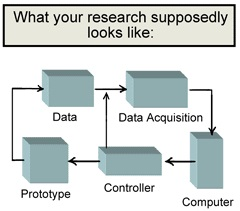
\includegraphics[width=8cm]{figuras/figura-1}}
	}{
	\Fonte{Estimote}			
}	
\end{figure}

\indent Os beacons são considerados dispositivos integrantes da próxima geração da internet, chamada de internet das coisas, onde terão um papel fundamental na forma de comunicação entre as mais variadas instituições como: lojas de varejo, locais de eventos, supermercados, restaurantes e instituições de ensino; e as pessoas. \\
\indent Entre os padrões de beacons existentes atualmente no mercado, dois se destacam por serem desenvolvidos pelas duas empresas -- Apple e Google -- mais importantes e inovadoras da área tecnológica. A seguir, os padrões serão explicados com detalhes. 


\subsection{iBeacon}
\label{sec:ibeacon}

\begin{quote}
O iBeacon é uma nova tecnologia que estende os Serviços de Localização no iOS. Seu dispositivo iOS pode alertar apps quando você se aproxima ou sai de um local com um iBeacon. Além de monitorar um local, o app pode estimar sua proximidade a um iBeacon (por exemplo, uma vitrine ou caixa em uma loja). Em vez de usar latitude e longitude para definir o local, o iBeacon usa um sinal de baixa energia de Bluetooth, detectado pelos dispositivos iOS. \cite{Apple}
\end{quote}

Esta tecnologia foi introduzida pela Apple a partir do seu sistema iOS versão 7, através dela as aplicações podem reagir aos sinal de beacons próximos ao dispositivo do usuário. Para isso o iBeacon envia pequenos pacotes de dados contendo o seu ID e a força de sinal. Como podemos ver abaixo:

\begin{quadro}[h!]	
	\centering
	\Caption{\label{qua:iBeacon-ID} Informações presentes em um pacote de sinal em iBeacons}		
	\UECEqua{}{
		\begin{tabular}{|c|c|l|}
			\hline
			Campo & Tamanho & Descrição \\
			\hline
			UUID & 16 bytes & Número identificador de um conjunto de beacons\\
			\hline
			Major & 2 bytes & Usado para identificar um subconjunto de beacons dentro do conjunto de beacons\\
			\hline
			Minor & 2 bytes & Usado para identificar individualmente um beacon dentro de um subconjunto\\				
			\hline
		\end{tabular}
	}{
	\Fonte{Elaborado pelo autor}
}
\end{quadro}

Os valores contidos no pacote são utilizados de maneira hierárquica pelo sistema iOS para determinar o beacon que o usuário está próximo.

\begin{quadro}[h!]	
	\centering
	\Caption{\label{qua:iBeacon-ID} Hierarquização de informações em iBeacons}		
	\UECEqua{}{
		\begin{tabular}{|c|c|c|c|c|}
			\hline
			\multicolumn{2}{|l|}{Localização} & Manaus & São Paulo & Rio de Janeiro \\
			\hline
			\multicolumn{2}{|l|}{UUID} & \multicolumn{3}{|c|}{AAAAAAAA-BBBB-CCCC-DDDD-EEEEEEEEEEEE}\\
			\hline
			\multicolumn{2}{|l|}{Major} & 1 & 2 & 3\\
			\hline
			\multirow{3}{4em}{Minor} & Bebidas & 10 & 10 & 10\\
			& Higiene & 20 & 20 & 20\\
			& Limpeza & 30 & 30 & 30\\				
			\hline
		\end{tabular}
	}{
	\Fonte{Elaborado pelo autor}
}
\end{quadro}
 
 No quadro acima, está exemplificado o caso envolvendo uma empresa com filiais em três cidades: Manaus, São Paulo e Rio de Janeiro. As três filiais compartilham o mesmo UUID que identifica de forma única a empresa. A identificação de cada filial fica sob responsabilidade do Major; no exemplo 1 para Manaus, 2 para São Paulo e 3 para Rio de Janeiro; E a identificação de cada setor dentro das filiais fica sob responsabilidade do Minor, no exemplo 10 para Bebidas, 20 para Higiene e 30 para Limpeza.
 
 \begin{figure}[h!]
 	\centering
 	\Caption{\label{fig:exemplo-2} Dinâmica do padrão iBeacon}	
 	\UECEfig{}{
 		\fbox{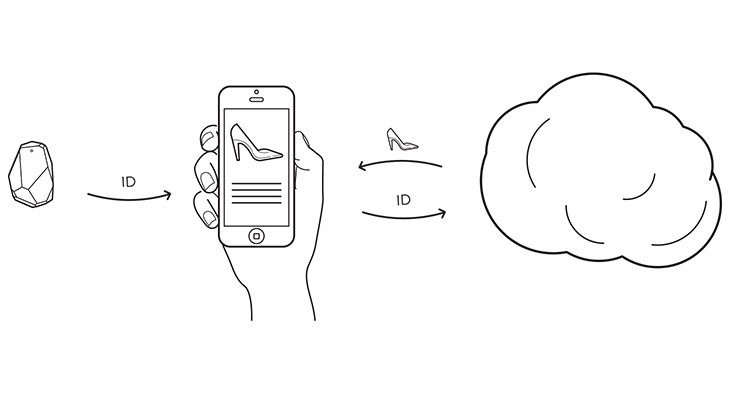
\includegraphics[width=8cm]{figuras/figura-2}}
 	}{
 	\Fonte{Estimote}			
 }	
\end{figure}
 
 \indent Segundo \cite{AppleInsider} iBeacons estão presentes em todas as lojas oficiais da Apple nos Estados Unidos. Através da utilização da aplicação oficial da loja e os iBeacons, os clientes podem ter acesso a uma camada extra de informações e serviços disponíveis nas lojas.
 
 \subsection{Eddystone}
 \label{sec:eddystone}
 
 Eddystone é um formato de beacon aberto do Google e que funciona com os sistemas Android e iOS. Eddystone inclui três tipos de estrutura para transmissão de dados, adequados para diferentes cenários. \cite{Google} \\
 \indent O padrão Eddystone é uma parte integrante da plataforma de beacons da Google. Com sua utilização é possível:
 
 \begin{itemize}
 	\item Permitir que as aplicações reajam ao contexto do usuário através de anexos (attachments) beacons;
 	\item Monitorar o status de uma frota de beacons a estrutura de telemetria do padrão Eddystone;
 	\item Transmitir dados para utilização da Web Física.
 \end{itemize}
 
 \begin{figure}[h!]
 	\centering
 	\Caption{\label{fig:exemplo-3} Dinâmica do padrão Eddystone}	
 	\UECEfig{}{
 		\fbox{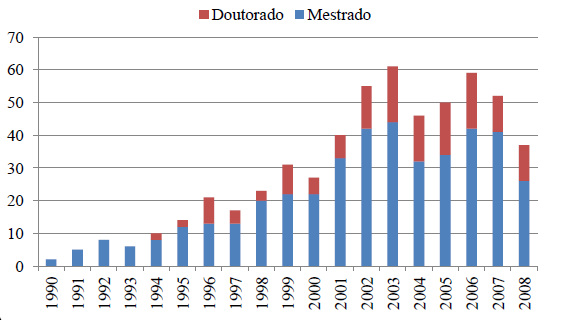
\includegraphics[width=8cm]{figuras/figura-3}}
 	}{
 	\Fonte{Google Developers}			
 }	
\end{figure}

A plataforma de beacons do Google é composta pelos próprios beacons, pelo padrão Eddystone e pela API de proximidade de beacons. \\
\indent Os beacons que suportam as especificações do padrão Eddystone podem transmitir dados de um único tipo de estrutura ou intercalar entre uma estrutura e outra. Por exemplo, transmitir repetidamente 50 estruturas do tipo Eddystone-UID seguidas de uma estrutura Eddystone-TLM. \\
\indent O padrão Eddystone especifica atualmente três tipos de estruturas: Eddystone-UID, Eddystone-URL e Eddystone-TLM.

\subsubsection{Eddystone-UID}
\label{sec:eddystone-uid}

Eddystone-UID contém o número identificador do beacon, que pode ser utilizado por um aplicação para disparar uma ação para o usuário. No Eddystone-UID, assim como ocorre no iBeacon, também é enviado um pequeno pacote de dados contendo um namespace e instance, detalhes no quadro abaixo:

\begin{quadro}[h!]	
	\centering
	\Caption{\label{qua:eddystone-UID} Informações presentes em um pacote de sinal em Eddystone}		
	\UECEqua{}{
		\begin{tabular}{|c|c|l|}
			\hline
			Campo & Tamanho & Descrição \\
			\hline
			Namespace & 10 bytes & Identificador de um conjunto de beacons\\
			\hline
			Instance & 6 bytes & Usado para identificar individualmente um beacon\\
			\hline
		\end{tabular}
	}{
	\Fonte{Elaborado pelo autor}
}
\end{quadro}

Para gerar um namespace a especificação do padrão Eddystone recomenda utilizar os dez primeiros bytes do hash SHA-1 gerado a partir de um nome de domínio. Exemplo de namespace gerado a partir do domínio ``fucapi.br'' utilizando a linguagem python:

\begin{figure}[h!]
	\centering
	\Caption{\label{fig:codigo-3} Código de exemplo para geração de namespace em python}	
	\UECEfig{}{
		\fbox{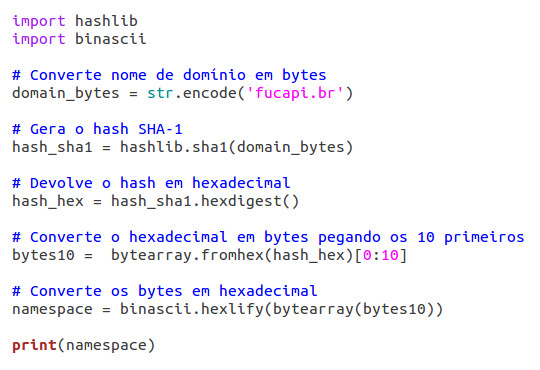
\includegraphics[width=8cm]{figuras/namespace_python}}
	}{
	\Fonte{Elaborado pelo autor}			
}	
\end{figure}

Ao executar o código a saída é:\\
\indent 1755ba6780003245d85c

\subsubsection{Eddystone-URL}
\label{sec:eddystone-url}

Eddystone-URL é a base para um novo conceito criado pela Google, chamado de Web Física, onde o usuário não precisará de um aplicativo dedicado para interpretar e executar as ações ao utilizar beacons fixados em objetos do mundo real. O conteúdo transmitido pelos beacons segue o mesmo padrão das URLs interpretadas pelos navegadores web, assim o usuário poderá acessar o conteúdo -- em forma de webapp ou website -- sem precisar baixar e instalar um aplicativo dedicado.

\subsubsection{Eddystone-TLM}
\label{sec:eddystone-tlm}

Eddystone-TLM especifica uma estrutura apropriada para transmissão de dados sobre os próprios beacons, permitindo que os mesmos possam ser gerenciados. Essa estrutura pode ser enviada juntamente com Eddystone-UID ou Eddystone-URL. A aplicação utilizada pelo usuário deve ser preparada para retransmitir os dados enviados pelo Eddystone-TLM para um serviço externo responsável por prover dados de gerenciamento. \\
\indent A estrutura pode conter os seguintes dados sobre os beacons:      

\begin{itemize}
	\item Tensão da bateria, que pode ser usado para estimar o nível de bateria restante em um beacon;
	\item Temperatura do beacon;
	\item Número de pacotes enviados desde a última vez que o beacon foi ligado ou reiniciado;
	\item Tempo de atividade desde a última vez que o beacon foi ligado ou reiniciado.
\end{itemize}

\section{Raspberry Pi}
\label{sec:raspberrypi}

De acordo com a \cite{RPiFoundation} Raspberry Pi é um microcomputador de dimensões mínimas, semelhante ao tamanho de um cartão de crédito, que pode ser conectado a um monitor e usa teclado e mouse padrão. \\

\begin{figure}[h!]
	\centering
	\Caption{\label{fig:raspberrypi} Raspberry Pi}	
	\UECEfig{}{
		\fbox{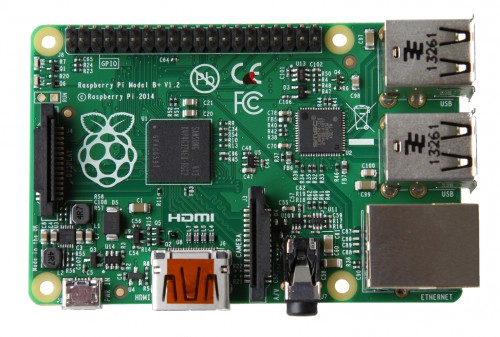
\includegraphics[width=8cm]{figuras/raspberrypi}}
	}{
	\Fonte{Raspberry Pi Foundation}			
}	
\end{figure}

Apesar de ser um microcomputador, é possível realizar a maioria das atividades da mesma forma que são realizadas em um computador pessoal convencional. Como navegar na internet, ouvir arquivos de audio e visualizar videos, criar documentos de textos, planilhas e apresentações. Raspberry Pi é desenvolvido pela Raspberry Pi Foundation, instituição que tem como principal objetivo, promover o estudo da ciência da computação e assuntos relacionados. \\
\indent Atualmente, em sua mais nova versão -- Raspberry Pi 2, é possível utilizar tanto sistema Linux, quanto Windows. Oficialmente é fornecida uma distribuição baseada no linux Debian chamada Raspbian, no caso do Windows a própria Microsoft disponibiliza uma versão adaptada do Windows 10, chamada Windows 10 IoT (Internet of Things). \\
\indent Além das dimensões mínimas, suas principais características estão relacionadas ao processador, armazenamento e porta GPIO (General Purpose Input/Output). O processador é baseado na arquitetura ARM, a mesma presente nos processadores de smartphones e tablets, o que proporciona baixo consumo de energia e também baixo aquecimento ao ponto de não necessitar de um dissipador de calor. O armazenamento de dados, inclusive do sistema operacional, é feito através do uso de um cartão SD, essa forma é muito vantajosa para realização de backup do sistema e também trocar ou alternar rapidamente o sistema utilizado no microcomputador. A porta GPIO é composta por um conjunto de pinos programáveis que são responsáveis pela comunicação de entrada e saída de sinais digitais, através dela é possível fazer comunicação com equipamentos externos ou periféricos. Como por exemplo LEDs, motores, sensores, entre outros.

\section{WiFi}
\label{sec:wifi}

Segundo \cite{Alecrim} WiFi é um conjunto de especificações para redes locais sem fio (WLAN - Wireless Local Area Network) baseada no padrão IEEE 802.11. O termo WiFi é um acrônimo de Wireless Fidelity, a Wifi Alliance é a instituição responsável por manter as especificações e certificar os produtos que utilizam esta tecnologia.\\
\indent A flexibilidade desta tecnologia é um fator de forte aderência para o mercado, pois através dela é possível conectar, formando uma rede, os mais variados tipos de dispositivos, como: smartphones, tablets, computadores, impressoras, TVs, Consoles de Jogos, Câmeras IP, entre outros. O uso mais comum da tecnologia WiFi é através do uso de roteadores sem fio para acesso à internet nos mais variados tipos de lugares, como: hotéis, restaurantes, aeroportos, bares, shoppings, universidades, praças públicas, entre outros.

\begin{figure}[h!]
	\centering
	\Caption{\label{fig:rede-wifi} Rede WiFi}	
	\UECEfig{}{
		\fbox{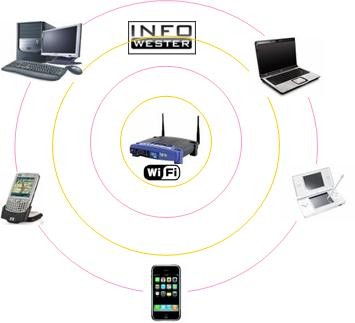
\includegraphics[width=8cm]{figuras/rede-wifi}}
	}{
	\Fonte{Infowester}			
}	
\end{figure}

Como mais de uma rede WiFi podem existir no mesmo lugar ou em lugares próximos, é preciso que as mesmas sejam identificadas com um SSID (Service Set Identifier) que consiste em um conjunto de até 32 caracteres. Popularmente é conhecido como ``nome'' da rede WiFi. \\
\indent Ao longo do tempo a Wifi Alliance tem mantido o padrão 802.11 em constante evolução, a cada nova versão é atribuída uma letra para efeito de representação. As diferenças básicas entre um padrão e outro estão relacionadas a três características principais: alcance de sinal, frequência de operação e velocidade de transmissão de dados.

\begin{quadro}[h!]	
	\centering
	\Caption{\label{qua:wifi-versoes} Versões do padrão 802.11}		
	\UECEqua{}{
		\begin{tabular}{|c|c|c|c|}
			\hline
			Versão & Alcance & Frequência & Velocidade \\
			\hline
			a & 35m & 5 GHz & 54 Mbps\\
			\hline
			b & 35m & 2.4 GHz & 11 Mbps\\
			\hline
			g & 38m & 2.4 GHz & 54 Mbps\\
			\hline
			n & 70m & 2.4/5 GHz & 74 Mbps\\
			\hline
		\end{tabular}
	}{
	\Fonte{Elaborado pelo autor}
}
\end{quadro}

\section{MQTT}
\label{sec:mqtt}

\begin{quote}
	MQTT é um protocolo de mensagens leve baseado em publicação/assinatura. Um ativador crítico de Internet of Things (IoT), o MQTT também pode ser usado para sistemas de mensagens corporativos confiáveis para dispositivos móveis, permitindo comunicações seguras, confiáveis, para a próxima geração de aplicativos móveis resilientes. \cite{Maynard}
\end{quote}

De acordo com \cite{MQTTorg} MQTT é um protocolo para conexão máquina a máquina ou para internet das coisas. Ideal para aplicações móveis devido ao seu tamanho pequeno, baixo consumo de energia, pacotes de dados minimizados e distribuição eficiente de informações para um ou mais receptores. Ele foi projetado para transportar mensagens com base no padrão publicador/assinante, ou seja, para o envio de uma mensagem existe o papel de um publicador e para o recebimento de uma mensagem existe um ou mais assinantes. Este padrão promove o desacoplamento entre as partes, pois publicador e assinante não conhecem a existência um do outro. Para isso é necessário um terceiro componente conhecido por ambos, chamado agente de mensagens, responsável por receber as mensagens referentes a um tópico do publicador e enviá-las aos assinantes que assinam o mesmo tópico de mensagem. O padrão publicador/assinante é uma alternativa ao tradicional padrão cliente-servidor, onde o cliente conhece e se comunica diretamente com o servidor. \\
\indent Suas principais características são:

\begin{itemize}
	\item Especificação aberta e de fácil adoção;
	\item Provê conectividade para dispositivos inteligentes através de mensagens;
	\item Oferece opções de conectividade otimizados para sensores e dispositivos remotos;
	\item Voltado para dispositivos com pouca memória e baixo poder de processamento;
	\item Ideal para redes limitadas com pouca largura de banda, alta latência e conexão instável;
	\item Promove escalabilidade na implantação e gerenciamento de soluções. 
\end{itemize}

Abaixo está uma simples representação da interação entre os atores envolvidos no padrão publicador-assinante.

\begin{figure}[h!]
	\centering
	\Caption{\label{fig:rede-wifi} Padrão Publicador-Assinante}	
	\UECEfig{}{
		\fbox{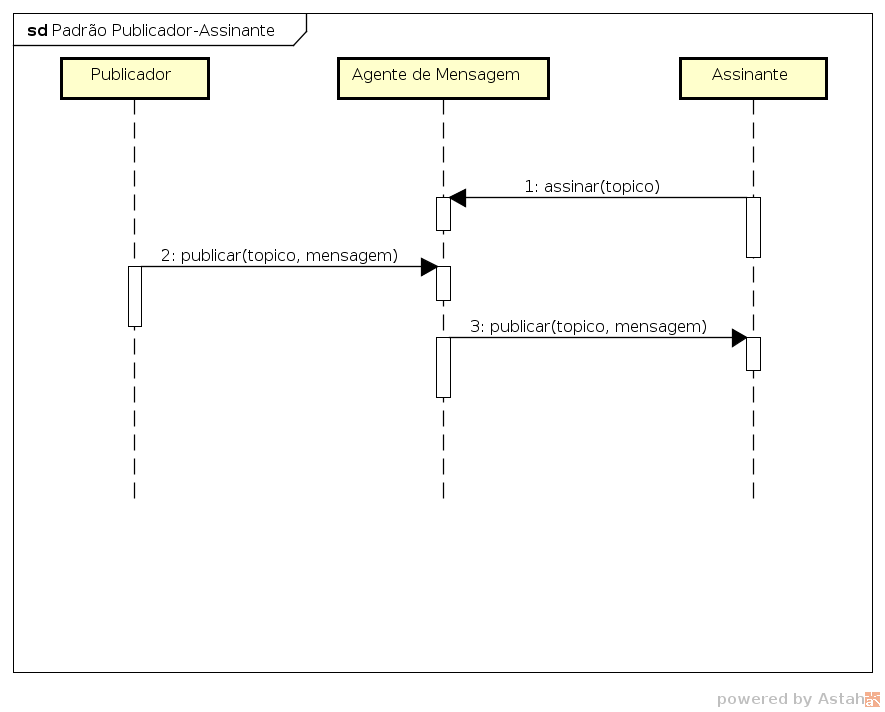
\includegraphics[width=8cm]{figuras/Publicador-Assinante}}
	}{
	\Fonte{Elaborado pelo Autor}			
}	
\end{figure}

\section{ActiveMQ}
\label{sec:activemq}

Segundo \cite{Posta} ActiveMQ é um serviço de mensageria de código aberto que pode servir como espinha dorsal para uma arquitetura de aplicações distribuídas baseadas em mensagens. \\
\indent Mensageria não representa somente uma forma de comunicação entre aplicações, mas também uma forma de integração entre elas. ActiveMQ implementa a Java Message Service (JMS) API, parte integrante da especificação J2EE, para permitir a criação, envio, recebimento e leitura de mensagens. Oferecendo uma solução de código aberto para comunicação assíncrona e de baixo acoplamento, provendo a integração das mais diferentes plataformas através da orientação a mensagens. \\
\indent ActiveMQ provê as seguintes características:

\begin{itemize}
	\item Conformidade com JMS -- Como já citado anteriormente, ActiveMQ é uma implementação da JMS API. O seu uso promove importantes benefícios, incluindo envio assíncrono de mensagem, modos de entrega persistente e não persistente, e durabilidade de mensagem para assinantes;
	\item Conectividade -- ActiveMQ possibilita conexão com uma ampla variedade de protocolos, incluindo HTTP/S, SSL, MQTT, STOMP, TCP, UDP e muitos outros;
	\item Persistência e Segurança -- ActiveMQ permite a configuração de suas opções para persistência e segurança. Por exemplo, a persistência de dados pode realizada via KahaDB, mas também pode ser modificada para realizar via JDBC. A autenticação pode utilizar o modo padrão via arquivo de propriedade ou o padrão JAAS;
	\item Desenvolvimento de aplicações usando Java -- O modo mais comum de desenvolver aplicações de envio e recebimento de mensagem utilizando ActiveMQ é utilizando Java;
	\item Integração com servidores de aplicação -- É possível integrar ActiveMQ com vários servidores de aplicação, como: Apache Tomcat, Tomee, Geronimo e JBoss;
	\item APIs Cliente -- Apesar de ActiveMQ implementar uma especificação da plataforma Java, através do uso de APIs cliente é possível desenvolver aplicações que utilizem ActiveMQ utilizando várias outras linguagens, como: C, C++, C\#, Perl, PHP, Python, Ruby e outras;
	\item Agrupamento de servidores -- É possível fazer que vários servidores rodando ActiveMQ possam trabalhar em conjunto formando um agrupamento de servidores. Essa opção geralmente é utilizada por motivos de escalabilidade;
	\item Administração simplificada -- Apesar de ActiveMQ ser destinado a desenvolvedores, um profissional de TI sem conhecimentos de programação pode facilmente utilizá-lo. Seu monitoramento por ser feito não somente através de seu console web, mas também utilizando JMX ou até mesmo via linhas de comando.  
\end{itemize}

\section{Servlet}
\label{sec:servlet}

Segundo a \cite{Oracle} servlet é uma classe da linguagem de programação Java que é utilizada para ampliar os recursos de servidores que hospedam aplicações acessadas por meio do modelo de programação solicitação-resposta. \\
\indent Embora servlet possa responder a qualquer tipo de solicitação, é muito comum a sua utilização no desenvolvimento de aplicações hospedadas em servidores web. Nesse caso, servlet define classes específicas para trabalhar com o protocolo HTTP. \\
\indent A classe HttpServlet define os métodos doGet e doPost para tratar as requisições para este protocolo. Sendo doGet recomendado para requisições que não alterem o estado da aplicação, como por exemplo uma consulta e o método doPost recomendado para enviar dados a serem processados, como ocorre em formulários HTML. Exemplo abaixo: \\

\begin{lstlisting}[language=Java,caption={Exemplo do método doGet}]
import java.io.IOException;
import java.io.PrintWriter;
import javax.servlet.ServletException;
import javax.servlet.http.HttpServlet;
import javax.servlet.http.HttpServletRequest;
import javax.servlet.http.HttpServletResponse;

public class HelloWorld extends HttpServlet {
	public void doGet(HttpServletRequest request, HttpServletResponse response) throws ServletException, IOException {
		PrintWriter out = response.getWriter();
		out.println("<html>\n" +
			"<head><title>Hello World</title></head>\n" +
			"<body>\n" +
			"<h1>Hello World</h1>\n" +
			"</body></html>");
	}
}
\end{lstlisting}

As classes HttpServletRequest e HttpServletResponse são utilizadas para acessar as informações de requisição e resposta respectivamente. Como no trecho de código abaixo: 

\begin{lstlisting}[language=Java,caption={Exemplo de uso HttpServletRequest}]
protected void doPost(HttpServletRequest request, HttpServletResponse response) throws ServletException, IOException { 
	String nome = request.getParameter("nome");
	String sobrenome = request.getParameter("sobrenome"); response.setContentType("text/html"); 
	PrintWriter out = response.getWriter(); out.println("Bem Vindo<h3>"+nome+" " +sobrenome+"</h3>"); 
	out.close(); 
}

\end{lstlisting}

O código fonte abaixo é utilizado para acessar o dispositivo de saída para a resposta:

\begin{lstlisting}[language=Java,caption={Acessando dispositivo de saída}]
PrintWriter out = response.getWriter();
\end{lstlisting}

\section{Kismet}
\label{sec:kismet}

Segundo \cite{Kershaw} é um analisador de rede, sniffer, e um sistema de detecção de intrusão. Kismet trabalha em conjunto com placas de rede que suportam o modo de monitoramento de rede, também chamado de modo promíscuo, que suportem os padrões 802.11a, 802.11b, 802.11g e 802.11n. Kismet é diferente das outras ferramentas de detecção porque trabalha em modo passivo, ou seja, ao invés de transmitir dados, somente escuta as transmissões. Quando o modo de monitoramento é ativado, a placa de rede fica indisponível para outras finalidades.\\
\indent Suas principais características são:

\begin{itemize}
	\item Trabalha em modo passivo coletando pacotes e detectando redes, inclusive redes com SSID oculto;
	\item Pode descobrir o canal de rede mais congestionado;
	\item Permite integração com GPS;
	\item O arquivo de captura de pacotes é compatível com outras ferramentas de análise de rede como Wireshark e Aircrack-ng;  
\end{itemize}

Kismet pode ser divido em trê partes: Drone, Servidor e Cliente. Kismet Drone pode ser utilizado para escutar pacotes de rede remotamente e enviá-los para um Kismet Servidor analisar os pacotes. Kismet Servidor pode trabalhar em conjunto com Kismet Drone ou sozinho, sua função é analisar os pacotes de rede. Kismet Cliente se comunica com Kismet Servidor para exibir as informações de redes e pacotes coletados.